\section{Antecedentes y Estado del Arte}

\subsection{2.1 Topologías DC-DC de Alta Eficiencia}

Particularmente llamativo resulta el ritmo acelerado con el que han evolucionado las topologías DC-DC en los últimos años. Mientras los convertidores buck y boost clásicos siguen dominando aplicaciones simples por su simplicidad, cada vez queda más claro que resultan insuficientes para los exigentes escenarios de los sistemas de potencia modernos.

Reddy et al. \cite{Reddy2025} ofrecen en su revisión una panorámica actualizada de las arquitecturas empleadas en movilidad eléctrica e integración de renovables. Sus hallazgos confirman que las topologías resonantes y de conmutación suave han ganado terreno de forma sostenida. Convertidores Dual Active Bridge (DAB), LLC, CLLC y sus variantes CLCLC destacan por permitir Zero Voltage Switching (ZVS) o Zero Current Switching (ZCS) en amplios rangos de operación, reduciendo drásticamente las pérdidas por conmutación.

No obstante, cabe matizar que muchas de estas soluciones exhiben compromisos difíciles de ignorar. Algunas alcanzan eficiencias muy altas solo en puntos de operación específicos, mientras que otras incrementan notablemente la complejidad del diseño magnético o elevan los costos de componentes.

\begin{table}[h]
\centering
\caption{Revisión comparativa de topologías DC-DC de alta eficiencia}
\label{tab:topologias}
\begin{tabular}{lcccc}
\hline
Topología & Eficiencia pico & Potencia típica & Bidireccional & Principales limitaciones \\
\hline
Buck/Boost tradicional & 92-95\% & <500 W & No & Altas pérdidas switching \\
DAB con SPS & 93-96\% & 1-10 kW & Sí & Circulantes elevados \\
LLC resonante & 95-97.5\% & 500 W-5 kW & Limitado & Rango estrecho \\
CLLC/CLCLC & 96-98.5\% & 1-20 kW & Sí & Diseño resonante complejo \\
Propuesta CLCLC optimizada & \textbf{>96\% amplio} & 1 kW & Sí & En evaluación \\
\hline
\end{tabular}
\end{table}

En muchos casos estudiados, la densidad de potencia y la robustez ante variaciones de carga siguen representando cuellos de botella importantes. Esta realidad motiva la búsqueda de configuraciones que no solo maximicen la eficiencia, sino que mantengan un comportamiento predecible en entornos dinámicos.

\subsection{2.2 Estrategias de Control Digital}

Uno de los desafíos persistentes que surge al analizar el control de convertidores DC-DC radica en equilibrar precisión, velocidad y robustez. Los métodos tradicionales basados en PI o PID, aunque ampliamente utilizados, tienden a mostrar limitaciones cuando las condiciones de operación se alejan del punto de diseño.

Resulta revelador observar cómo el control predictivo por modelo (MPC) ha emergido como alternativa prometedora. Guo et al. \cite{Guo2025_MPC} presentan recientemente un esquema unificado de MPC para convertidores buck que logra excelente seguimiento de referencia y rechazo de perturbaciones. Su enfoque destaca por reducir el horizonte de predicción manteniendo garantías de estabilidad, aspecto crítico en implementaciones embebidas.

Aun así, no todo son ventajas. El MPC clásico puede demandar una carga computacional elevada, lo que obliga a realizar compromisos entre frecuencia de muestreo y complejidad del modelo. Aquí es donde técnicas híbridas, que combinan MPC con modulación de fase múltiple, parecen ofrecer un camino intermedio atractivo. La modulación Triple Phase-Shift (TPS), por ejemplo, permite regular el flujo de potencia con mayor flexibilidad que la Single Phase-Shift convencional, aunque su implementación digital requiere cuidadosa sincronización.

\subsection{2.3 Aplicaciones en Microgrids y EPS}

Lejos de ser un asunto resuelto, la integración efectiva de convertidores DC-DC en microgrids y sistemas de potencia eléctricos continúa planteando interrogantes relevantes. Gronfula y Zellagui \cite{Gronfula2025} analizan las tendencias futuras en conversión DC-DC para renovables y subrayan la necesidad de soluciones que vayan más allá de la mera eficiencia punto a punto.

En entornos de microgrids DC, los convertidores deben gestionar flujos bidireccionales, coordinarse con baterías y responder a variaciones súbitas de generación y demanda. En este escenario, muchas propuestas existentes muestran debilidades: o bien sacrifican eficiencia para ganar dinamismo, o bien carecen de mecanismos de coordinación a nivel de sistema.

\begin{figure}[h]
\centering
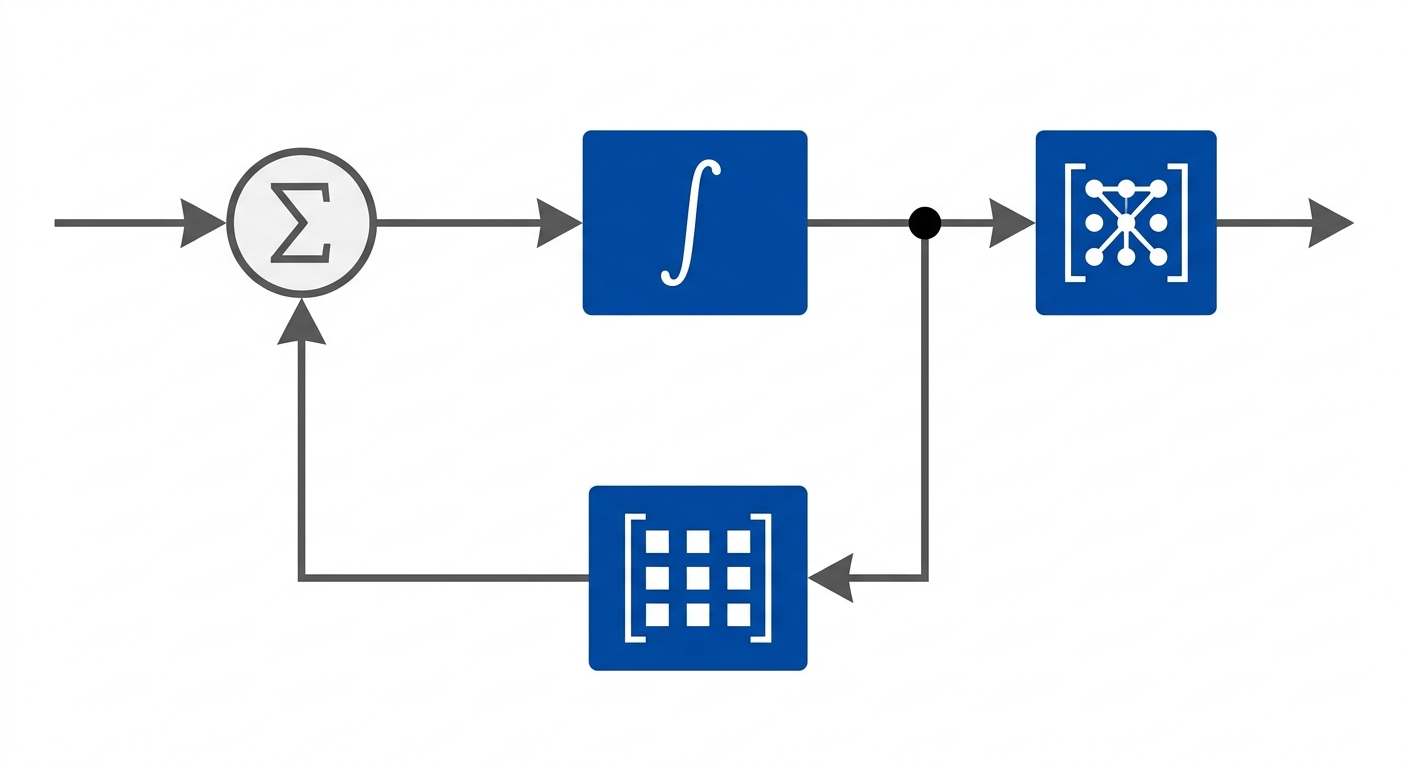
\includegraphics[width=0.92\linewidth]{fig2.png}
\caption{Evolución temporal de la eficiencia máxima reportada en convertidores DC-DC para aplicaciones en sistemas de potencia y microgrids (2018-2026).}
\label{fig:evolucion_eficiencia}
\end{figure}

La brecha identificada es clara: se requieren convertidores no solo eficientes, sino verdaderamente inteligentes, capaces de integrarse en estrategias de gestión energética distribuidas. Esta observación establece el fundamento para la propuesta que se desarrolla en las secciones siguientes, donde se busca cerrar precisamente estas limitaciones mediante una combinación cuidadosa de topología resonante avanzada y control digital predictivo.